\documentclass[a4paper]{report}
% Shared preamble for the English probability and statistics documents.
% Based on the original course preamble. Compile with pdfLaTeX.
\usepackage[top=1.5cm,bottom=2cm,left=2cm,right=2cm]{geometry}
\usepackage[T1]{fontenc}
\usepackage{lmodern}
\usepackage[utf8]{inputenc}
\usepackage[english]{babel}

\usepackage{amsmath}
\usepackage{amssymb}
\usepackage{amsthm}
\usepackage{mathrsfs}
\usepackage{mathtools}
\usepackage{etoolbox}
\usepackage{tikz}
\usetikzlibrary{shapes.multipart,arrows.meta}
\usepackage{xcolor}
\usepackage{enumerate}
\usepackage[shortlabels]{enumitem}
\usepackage{hyperref}
\usepackage{version}
\usepackage{bbold}
\usepackage{fontawesome5}
\usepackage{fancyhdr}
\lfoot{}
\usepackage{natbib}
\usepackage{graphicx}
\usepackage{pdfpages}
\usepackage{authblk}
    
\usepackage{blindtext}
\usepackage{multicol}
\usepackage{collcell}
\usepackage{wrapfig}
\usepackage{blkarray}
\usepackage{cancel}
\usepackage{appendix}
\usepackage{float}
\makeatletter
\input{tex/assets/slashbox.sty}
\makeatother
\hypersetup{unicode,colorlinks,citecolor=red,filecolor=black,
  linkcolor=red,urlcolor=cyan}
\setlength{\columnsep}{1cm}
\pagenumbering{gobble}

\def\numtext#1{%
  \ifcase#1\or one\or two\or three\or four\or five\or six\or seven\or eight\or nine\or ten\or
  eleven\or twelve\or thirteen\or fourteen\or fifteen\or sixteen\or seventeen\or eighteen\or nineteen\or twenty\or Lots\fi}

\newcommand{\Byte}[1]{%
  \def\nodecontents{}%
  \foreach[count=\l] \k in {#1} {\xappto{\nodecontents}{\noexpand\nodepart{\numtext{\l}}\k}}%
  \node[rectangle split,rectangle split parts=8,rectangle split horizontal,draw] at (2,2){\nodecontents};}

\newcommand{\D}{{\mathrm{d}}}
\newcommand{\cE}{{\mathcal{E}}}
\newcommand{\cG}{{\mathcal{G}}}
\newcommand{\cX}{{\mathcal{X}}}
\newcommand{\cY}{{\mathcal{Y}}}
\newcommand{\cB}{{\mathcal{B}}}
\newcommand{\cF}{{\mathcal{F}}}
\newcommand{\cO}{{\mathcal{O}}}
\newcommand{\cS}{{\mathcal{S}}}
\newcommand{\cT}{{\mathcal{T}}}
\newcommand{\given}{\, \big| \,}
\newcommand{\cL}{{\mathscr{L}}}
\newcommand{\cD}{{\mathcal{D}}}
\newcommand{\cA}{{\mathscr{A}}}
\newcommand{\cP}{{\mathscr{P}}}
\newcommand{\cR}{{\mathscr{R}}}
\newcommand{\A}{{\mathcal A}}
\newcommand{\one}{\mathbb{1}}
\newcommand{\mathbbm}[1]{\mathbb{#1}}

\providecommand{\C}{}
\renewcommand{\C}{\mathbb C}
\newcommand{\R}{\mathbb R}
\newcommand{\Q}{\mathbb Q}
\newcommand{\N}{\mathbb N}
\newcommand{\T}{\mathbb T}
\newcommand{\F}{\mathbb F}
\renewcommand{\P}{\mathbb P}
\newcommand{\Z}{\mathbb Z}
\newcommand{\E}{\mathbb {E}}
\newcommand{\Pbb}[1]{\P\left( #1\right)}
\newcommand{\Ebb}[1]{\E\left[ #1\right]}

\newcommand{\lb}{\left (}
\newcommand{\rb}{\right )}
\newcommand{\lbb}{\left [}
\newcommand{\rbb}{\right ]}
\newcommand{\labs}{\left |}
\newcommand{\rabs}{\right |}
\newcommand{\lbrb}[1]{\lb #1 \rb}
\newcommand{\lbbrbb}[1]{\lbb#1\rbb}
\newcommand{\labsrabs}[1]{\labs#1\rabs}
\newcommand{\lbbrb}[1]{\lbb#1\rb}
\newcommand{\lbrbb}[1]{\lb#1\rbb}
\newcommand{\langlerangle}[1]{\langle#1\rangle}
\newcommand{\lbcurly}{\{}
\newcommand{\rbcurly}{\}}
\newcommand{\curly}[1]{\lbcurly#1\rbcurly}
\newcommand{\abs}{\labsrabs}
\newcommand{\ind}[1]{1_{#1}}
\newcommand{\indep}{\perp \!\!\! \perp}
\renewcommand{\d}{\, \mathrm{d}}

\newtheorem{theorem}{Theorem}
\newtheorem{problemCnt}{Lemma}
\theoremstyle{definition}
\newtheorem{problem}[problemCnt]{Problem}
\newtheorem{problembook}[problemCnt]{\faBook \,  Problem}
\newtheorem{problempencil}[problemCnt]{\faPencil* \,  Problem}
\newtheorem{problemstar}[problemCnt]{\faStar\,  Problem}
\newtheorem{problemstarpencil}[problemCnt]{\faStar \, \faPencil* \,   Problem}
\newtheorem{probleminteresting}[problemCnt]{\faSmile[regular] \,   Problem}
\newtheorem{solution}{Solution}

\newcommand{\fwcell}[1]{\makebox[\arraystretch\normalbaselineskip]{$#1$}}
\newenvironment{enumeratei}{\begin{enumerate}[(i)]}{\end{enumerate}}
\newenvironment{enumeratea}{\begin{enumerate}[(a)]}{\end{enumerate}}
\newenvironment{enumeraten}{\begin{enumerate}[\upshape 1.]}{\end{enumerate}}

% Compatibility helpers needed by a few files in the combined archive.
\AtBeginDocument{\noindent{\footnotesize English translation prepared with ChatGPT (OpenAI, GPT-6), 26 October 2026, for translation of the Bulgarian text into English and LaTeX formatting.
The Bulgarian originals remain the reference; translation may contain errors.}\par\smallskip}
\newcommand{\MissingGraphic}[1]{%
  \begin{center}\fbox{\parbox{0.82\linewidth}{\centering Missing source image: \texttt{#1}}}\end{center}}



\begin{document}
\noindent Probability and Statistics, CS Year 3, Stream 2 \hfill Written examination, 2 July 2023
\hrulefill
\begin{problem}
A speed-measuring device's percentage error has distribution $N(0,5^2)$.
\begin{enumerate}
\item (0.25 points) On average, how many cars pass before the first error of at least 10\%? Among 1000 cars, how many errors exceed 10\% on average? After 100 cars, what is the probability that the mean error exceeds 1\%?
\item (0.25 points) Model passing speeds in km/h as independent $N(40,5^2)$ variables. What is the probability that the device records a speed above the 50 km/h limit? What must its standard deviation be for the mean error after 100 cars to exceed 1 km/h with probability 0.1\%?
\item (0.5 points) Answer part 1 using absolute error, the modulus of the error in that part.
\end{enumerate}
\end{problem}
\begin{problem}
A travel company advertises seaside hotels by repeatedly calling $N\sim\mathrm{Poi}(\lambda)$ contacts. Person $i$ accepts after $K_i$ calls, where the $K_i$ are iid, independent of $N$, with $\P(K_i=n)=f(n)$. The value $\infty$ is allowed, so $f(\infty)\geq0$. Let $X_n=\sum_{i=1}^N\mathbbm1_{\{K_i=n\}}$ count holidays sold in round $n$.
\begin{enumerate}
\item (0.5 points) Prove that the $X_n$ are independent and $X_n\sim\mathrm{Poi}(\lambda f(n))$.
\item (0.5 points) The company stops after $T=\inf\{n:X_n=0\}$, the first round with no new customer. Let $S=X_1+\cdots+X_T$. Prove $\E[S]=\lambda\E[F(T)]$, where $F(k)=f(1)+\cdots+f(k)$.
\end{enumerate}
\end{problem}
\begin{problem}
Let $U\sim U(0,1)$ and $V\sim U(-\pi/2,\pi/2)$.
\begin{enumerate}
\item (0.5 points) One method of generating a pseudorandom number between 0 and 1 from $U$ chooses a usually large positive integer $M$ and takes $X=\{MU\}$, the fractional part. Find $\E X$, $DX$ and $\mathrm{Cor}(U,X)$. What do you think of this method?
\item (0.5 points) Let $U_1,\ldots,U_{100}$ be iid copies of $U$. Find their individual expectations and those of the maximum and minimum.
\item (0.5 points) Find the density, expectation and variance of $Y=\tan V$.
\item (0.5 points) For $Z\sim\mathrm{Cauchy}(1)$ with density $1/[\pi(1+x^2)]$, prove that $1/Z$, $2Z/(1-Z^2)$ and $(3Z-Z^3)/(1-3Z^2)$ have the same distribution.
\end{enumerate}
\end{problem}
\noindent\textbf{Bonus}
\begin{enumerate}
\item (0.25 points) Define $D(Y\mid X)=\E[(Y-\E[Y\mid X])^2\mid X]$. Recall $\E X=\E[\E[X\mid Y]]$. Which of
\[\E[D(Y\mid X)],\quad D(D(Y\mid X)),\quad\E[D(Y\mid X)]+D(D(Y\mid X)),\]
\[\E[D(Y\mid X)]+D(\E[Y\mid X])\]
expresses $DY$ in terms of conditional variance?
\end{enumerate}
Construct Cantor's function $c:[0,1]\to[0,1]$ recursively: $f(x)=1/2$ on $[1/3,2/3]$, $f(x)=f(3x)/2$ on $[0,1/3)$, and $f(x)=(1+f(3x-2))/2$ on $(2/3,1]$.
\begin{figure}[ht]\centering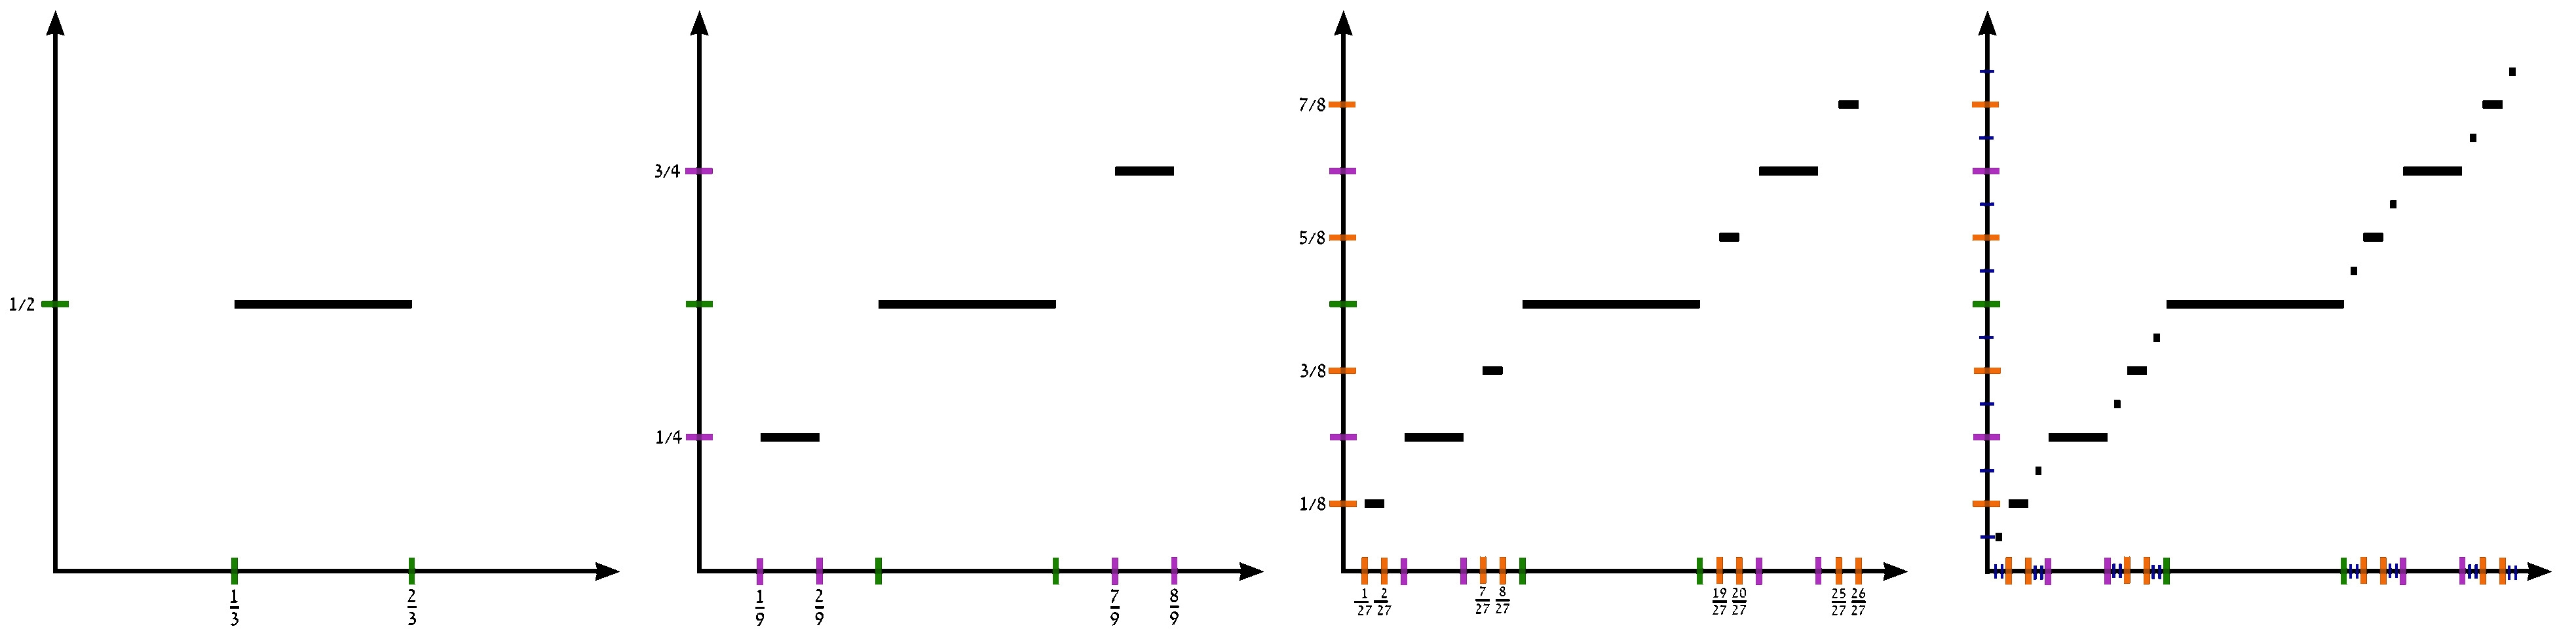
\includegraphics[width=\textwidth]{tex/assets/prob-stat/Cantor.jpg}
\caption{Recursive construction of Cantor's function. Source: \href{https://en.wikipedia.org/wiki/Cantor_function}{Wikipedia}.}\end{figure}
\begin{enumerate}[start=2]
\item (0.25 points) Let $F_X(x)=c(x)$ for $x\in(0,1)$. Find $\E X$ and $DX$.
\item (0.25 points) Prove that $F_X$ is differentiable almost everywhere. What is the density $f_X$?
\end{enumerate}
\end{document}
